% Kapitel 4
%-------------------------------------------------------------------------------
\chapter{Verteilungsentwurf}
Da es sich bei dem Produkt um eine Datenbank-basierte Webanwendung handelt, liegt hier ein verteiltes System in Form eines Client-Server-Modells vor:

\begin{figure}[h]
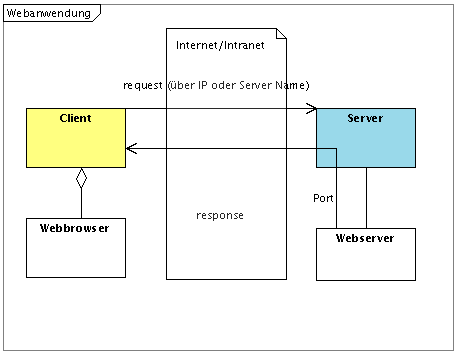
\includegraphics[width=0.8\linewidth]{bilder/Webanwendung2.png}
\caption{Client-Server-Modell}
\label{Client-Server-Modell}
\end{figure}

Durch eine Ressource-Anforderung (request) mithilfe eines Webbrowsers benutzt der Client über eine IP (oder einem Servernamen) die Adresse des Servers. Dieser gibt den Request an den Webserver weiter.
Mithilfe des Servers beanwortet der Webserver schließlich den Request und schickt das Ergebnis (response) an den Client zurück.   

